
%----------------------------------------------------------------------------------------
%	PACKAGES AND DOCUMENT CONFIGURATIONS
%----------------------------------------------------------------------------------------

\documentclass{article}

%\usepackage{mhchem} % Package for chemical equation typesetting
%\usepackage{siunitx} % Provides the \SI{}{} command for typesetting SI units
\usepackage[T1]{fontenc}
\usepackage[utf8]{inputenc}
%
\usepackage[swedish]{babel}
\usepackage{graphicx} % Required for the inclusion of images
\usepackage{float}
\usepackage{caption}
\usepackage{subcaption}

%Matte
\usepackage{amsmath}
\usepackage[makeroom]{cancel}
\usepackage{gensymb} % \degree

\setlength\parindent{0pt} % Removes all indentation from paragraphs
%\renewcommand{\labelenumi}{\alph{enumi}.} % Make numbering in the enumerate environment by letter rather than number (e.g. section 6)
%\usepackage{times} % Uncomment to use the Times New Roman font

%%% För kod!
\usepackage{listingsutf8}
\usepackage{color}
\definecolor{dkgreen}{rgb}{0,0.6,0}
\definecolor{gray}{rgb}{0.5,0.5,0.5}
\definecolor{mauve}{rgb}{0.58,0,0.82}
\lstset{frame=tb,
  language=Matlab,
  aboveskip=3mm,
  belowskip=3mm,
  showstringspaces=false,
  columns=flexible,
  basicstyle={\small\ttfamily},
  numbers=none,
  numberstyle=\tiny\color{gray},
  keywordstyle=\color{blue},
  commentstyle=\color{dkgreen},
  stringstyle=\color{mauve},
  breaklines=true,
  breakatwhitespace=true
  tabsize=3
  extendedchars=\true,
  inputencoding=utf8/latin1
}
%%%% slut kod



%----------------------------------------------------------------------------------------
%	DOCUMENT INFORMATION
%----------------------------------------------------------------------------------------

\title{Elteknik - inlämning 1} % Title

\author{
	\begin{tabular}{l r}
    Marcus Olsson \\
    %number & number & number% Author name
    \\
    \end{tabular}
    }

\date{\today} % Date for the report

\begin{document}

\maketitle % Insert the title, author and date
\tableofcontents
\clearpage
%----------------------------------------------------------------------------------------
%	SECTION 1
%----------------------------------------------------------------------------------------
\section{intro}
Beräkningar är gjorda i MATLAB och koden finns i Appendix.

%----------------------------------------------------------------------------------------
%	SECTION 2
%----------------------------- -
\section{A}
Ett litet elnät planeras med följande laster vid 400V

\begin{enumerate}
	\item Flerfamiljehus – den beräknade toppeffekten är 250 kW, $cos\varphi = 0,98$.
	\item Förskola och andra samlingslokaler – effektbehovet max 100 kVA, $cos\varphi = 0,95$
	\item En symmetrisk trefas, Y – kopplad asynkronmotor med märkspänning 400 V,
märkström 200 A och $cos\varphi = 0,8$. Parallellt med motorn är ett kondensatorbatteri
inkopplat som är märkt 90 kVAr.
\end{enumerate}

\subsection{a}
Här ska fasströmmen som respektive last drar beräknas.
Ett visardiagram skall ritas för varje ström samt den totala strömmen, fas a används som referens.
Ekvikalenta impedanser skall också beräknas.
Här antas symmetriska laster.

  \subsubsection{Fasströmmar}
  Effekten i flerfamiljehuset är 250kW, eftersom enheten är watt är det aktiv effekt som är beräknat.
  Jag använder [\ref{P}] för att beräkna strömmen $I_1$ där $U=400\angle{0\degree}$
  Detta ger mig $I_1=xx=a+jb$

  \begin{equation}
    P=\sqrt3UIcos\varphi
    \label{P}
  \end{equation}

  Effekten för förskolan är skriven i Voltampere, detta betyder att det är skenbar effekt som är beräknat.
  Då använder jag [\ref{S}] och löser ut $I_2$ för att få fram att $I_2=(I_2^*)^*=xx=a+jb$

  \begin{equation}
    S=\sqrt3UI^*=P+jQ
    \label{S}
  \end{equation}

  Motorn är parallellkopplad med ett kondensatorbatteri för att faskompenseras och därmed dra en lägre total reaktiv effekt.
  Här används [\ref{Q},\ref{P},\ref{S}] för att få fram aktiv och reaktiv effekt för motorn.
  Effekterna kan sedan summeras eftersom de är parallellkopplade för att få fram den totala skenbara effekten.
  Efter detta kan jag göra precis som i förra upgiften för att lösa ut $I_2=xx\angle{xx\degree}=a+jb$

  \begin{equation}
    Q=\sqrt3UIsin\varphi
    \label{Q}
  \end{equation}

  När dessa är beräknade så kan man enkelt räkna ut den totala strömmen genom att summera de enskilda komplexa strömmarna.
  Detta ger $I_{tot}=xx$

  %Infoga bilder på visardiagrammen.
  \subsubsection{Impedanser}
  De ekvivalenta impedanserna fås ur Ohms lag [\ref{ohms}], dessa blir följande:
  \begin{equation}
    Z=\frac{U}{I}
    \label{ohms}
  \end{equation}

  %Infoga tabell med ekvivalenta impedanser

\subsection{b}
  Här ska den skenbara effekten beräknas, för alla laster inkopplade och var och en för sig.
  Ekvation [\ref{S}] används för de olika lasterna och då fås följande resultat.
  Eftersom vinkeln för $S_{tot}$ är positiv så är den totala lasten induktiv.

  \begin{tabular}{l}
      $S_1=250 + j29.3 kVa$ \\
      $S_2=100kVA$ \\
      $S_311.1e - j6.86 kVA$\\
      $S_{tot}=461 + j22.4 kVa$
  \end{tabular}

\subsection{c}
Den tredje lasten är faskompenserad med ett kondensatorbatteri.
Detta gör man ofta på större motorer för att minska den reaktiva effekten i nätet.

%----------------------------------------------------------------------------------------
%	SECTION 3
% %----------------------------------------------------------------------------------------
\section{B}
  En osymmetrisk trefas är kopplad till en huvudspänning på $U_{ab}=400V$
  Fasströmmarna samt strömmen genom varje impedans skall beräknas.
  Ett visardiagram skall också ritas med $U_{ab}$ som referens.
  \\
  \\
  Jag börjar med att sätta ut referenser för strömmarna enligt Figur \ref{fig:osymm} och använder Ohms lag [\ref{Ohms}]\
   med spänningarna $U_1=400\angle{0\degree},U_2=400\angle{-120\degree},U_3=400\angle{-240\degree}$ för att beräkna strömmarna över varje last.
  Efter detta använder jag KCL enligt nedan för att få fram fasströmmarna.

  \begin{tabular}{| l}
    $I_a=I_{ab}+I_{ac}=xx$\\
    $I_b=I_{bc}-I_{ab}$\\
    $I_c=-(I_{bc}+I_{ac})$\\
  \end{tabular}

  \begin{figure}[H]
  \begin{center}
  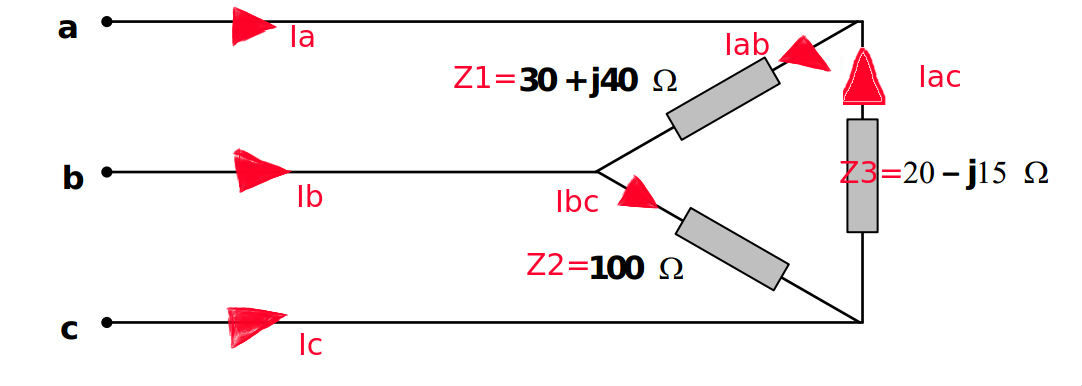
\includegraphics[width=1\textwidth]{img/osymmetrisk-last1.jpg} % Include the image placeholder.png
  \caption{Osymmetrisk last med strömreferenser inritade}
  \label{fig:osymm}
  \end{center}
  \end{figure}


%----------------------------------------------------------------------------------------
%	SECTION 4
%----------------------------------------------------------------------------------------
\section{C}
\subsection{a}
lorem
\subsection{b}
ipsum
%----------------------------------------------------------------------------------------
%	SECTION 5
%----------------------------------------------------------------------------------------
\section{D}
\subsection{a}
lorem
\subsection{b}
ipsum
\subsection{c}
lorem
\subsection{d}
lorem
\subsection{e}
lorem
\subsection{f}
lorem
\subsection{g}
lorem
\subsection{h}
lorem
\subsection{i}
%----------------------------------------------------------------------------------------
%	SECTION 6
%----------------------------------------------------------------------------------------


%----------------------------------------------------------------------------------------
%	SECTION 7
%----------------------------------------------------------------------------------------


%----------------------------------------------------------------------------------------
%	SECTION 8
%---------------------------------------------------------------------------------------


%----------------------------------------------------------------------------------------
%	SECTION 9
%----------------------------------------------------------------------------------------


%----------------------------------------------------------------------------------------
%	SECTION 10
%----------------------------------------------------------------------------------------


%-----------------------------------------------------------------------------
%	Appendix
%-----------------------------------------------------------------------------
 \newpage
 \appendix
 \section{Matlab}

 \lstinputlisting[label=main.m,caption=main.m]{code/main.m}

% \subsection{Images}

% \begin{figure}[H]
% \begin{center}
% \includegraphics[width=1\textwidth]{img/bode.jpg} % Include the image placeholder.png
% \caption{Bode}
% \end{center}
% \end{figure}


%----------------------------------------------------------------------------------------
%	BIBLIOGRAPHY
%----------------------------------------------------------------------------------------

%\bibliographystyle{unsrt}

%\bibliography{sample}

%----------------------------------------------------------------------------------------


\end{document}
